

\documentclass{beamer}



\mode<presentation> {
\usetheme{Luebeck}
\usecolortheme{whale}
}

\usepackage{graphicx} % Allows including images
\usepackage{booktabs} % Allows the use of \toprule, \midrule and \bottomrule in tables
\usepackage{gensymb}
\usepackage{amsmath}

%----------------------------------------------------------------------------------------
%	TITLE PAGE
%----------------------------------------------------------------------------------------

\title[Low Thrust Interplanetary Trajectory Optimization using DE]{Low Thrust Interplanetary Mission Trajectory Optimization using Differential Evolution} % The short title appears at the bottom of every slide, the full title is only on the title page

\author[Padmanbha Prasanna Simha, Ramanan R. V (IIST)]{Padmanabha Prasanna Simha\\Ramanan R. V} % Your name
\institute[IIST] % Your institution as it will appear on the bottom of every slide, may be shorthand to save space
{
Indian Institute of Space Science and Technology \\ for\\ National Conference on Multidisciplinary Design, Analysis and Optimization\\ (Indian Institute of Science - Bangalore)% Your institution for the title page
\medskip
%\textit{(padmanabhapsimha@gmail.com)\\(padmanabha.sc14b034@ug.iist.ac.in)
%	\\(rvramanan@iist.ac.in)} % Your email address
}
\date{March 24, 2018} % Date, can be changed to a custom date

\begin{document}

\begin{frame}
\titlepage % Print the title page as the first slide
\end{frame}

%\begin{frame}
%\frametitle{Overview} % Table of contents slide, comment this block out to remove it
%\tableofcontents % Throughout your presentation, if you choose to use \section{} and \subsection{} commands, these will automatically be printed on this slide as an overview of your presentation
%\end{frame}

%----------------------------------------------------------------------------------------
%	PRESENTATION SLIDES
%----------------------------------------------------------------------------------------

%------------------------------------------------
%\section{Abstract} % Sections can be created in order to organize your presentation into discrete blocks, all sections and subsections are automatically printed in the table of contents as an overview of the talk
%------------------------------------------------
\section{Problem Definition}

\begin{frame}
\frametitle{Interplanetary Transfers with Electrically Propelled Spacecraft}
\begin{itemize}
	\vspace{-3mm}
	\item Electric propulsion offers a good option for interplanetary transfers.
	\pause
	\item Spacecraft in initial heliocentric orbit.
	\pause
	\item To rendezvous with a final heliocentric orbit under heliocentric gravitational dynamics.
	\pause
	\item Thrust vector magnitude and direction are the control variables that are to be determined to optimize:
	\begin{itemize}
		\item Flight duration
		\item Propellant consumption
	\end{itemize}
	\pause
	\item Only gradual velocity changes are possible due to low thrust.
	\pause
	\item Coasting is to be allowed and should arise naturally out of the solution.
	\pause
	\item Indirect approach to optimal control has been followed to solve this problem.
\end{itemize}
\end{frame}


\begin{frame}
	\frametitle{Electric propulsion (EP) power-plant types considered}
	\begin{itemize}
		\item Nuclear electric propulsion (NEP) 
		\begin{itemize}
			\item Constant power availability
		\end{itemize}
		\item Solar electric propulsion (SEP)
		\begin{itemize}
			\item Inverse square law model (first approximation to available power)
			\item Williams and Coverstone-Carroll model (from experimental data)
		\end{itemize}
	\end{itemize}
\end{frame}


\section{Problem Formulation}
\begin{frame}
	\frametitle{Equations of motion}
	\begin{align}
		\dot{x}&=v_x\\
		\dot{y}&=v_y\\
		\dot{v}_x&=-\frac{\mu_s x}{r^3}+a_x\\
		\dot{v}_y&=-\frac{\mu_s y}{r^3}+a_y\\
		\dot{m}&=-\frac{m\sqrt{a_x^2+a_y^2}}{g_0I_{sp}}
	\end{align}
	The above equations govern both time and fuel optimal trajectories.
\end{frame}

\begin{frame}
\frametitle{Cost functions}
\begin{align}
J_{time}&=\Phi_f+\int\limits_{t_0}^{t_f}dt \hspace{25mm}\text{subject to}\hspace{5mm} m\sqrt{a_x^2+a_y^2}=T_{max}\\
J_{fuel}&=\Phi_f+\int\limits_{t_0}^{t_f}\frac{m\sqrt{a_x^2+a_y^2}}{g_0I_{sp}}dt \hspace{5mm}\text{subject to}\hspace{5mm} m\sqrt{a_x^2+a_y^2}\leq T_{max}
\end{align}
$\Phi_f$ represents the error in achieving the final desired orbit.
\end{frame}


\begin{frame}
	\frametitle{Two Point Boundary Value Problem (TPBVP) Formulation} 
	\vspace{-2.0mm}
	\begin{block}{TPBVP formulation}
		\vspace{-3mm}
		\begin{itemize}
		\item Costates are introduced and the Hamiltonian is formed
		\item System dynamics, cost functionals and costates form the Hamiltonians.
		\item Pontryagin's minimum principle gives the costate dynamics and the optimal control law.
		\item Initial costates are unknown.
		\item Problem is reduced to the determination of initial costates such that the final state is achieved with maximum accuracy.
		\end{itemize}
	\end{block}
	\vspace{-1.5mm}
	\begin{block}{Variables}
	\begin{itemize}
		\vspace{-3mm}
		\item States - $[x$ $y$ $v_x$ $v_y$ $m]$, Costates - $[\lambda_x$ $\lambda_y$ $\lambda_{v_x}$ $\lambda_{v_y}$ $\lambda_m]$
		\item Controls - $[a_x$ $a_y]$
	\end{itemize}
	\end{block}
\end{frame}

\begin{frame}
	\frametitle{Optimal Control Law with Constraints}
	\begin{itemize}
		\item Results in constrained minimization problem.
		\item Lagrange multipliers or the Karush-Kuhn-Tucker (KKT) conditions are utilized to obtain the control law.
	\end{itemize}
	\begin{align}
		&l=\frac{\sqrt{\lambda_{v_x}^2+\lambda_{v_y}^2}}{m}-\frac{1-\lambda_m}{g_0I_{sp}} \hspace{15mm} k=-\frac{T_{max}/m}{\sqrt{\lambda_{v_x}^2+\lambda_{v_y}^2}}\\
		&\text{Fuel optimal - }\left \{
		\begin{array}{ccc}
		\text{If } l\geq 0, &a_x=k\lambda_{v_x}  &a_y=k\lambda_{v_y}\\
		\text{If } l<0, &\hspace{-4mm}a_x=0  &\hspace{-4mm}a_y=0
		\end{array}
		\right.\\
		&\text{Time optimal - }a_x=k\lambda_{v_x}\hspace{4mm}a_y=k\lambda_{v_y}
	\end{align}
\end{frame}

\section{Solution Procedure}
\begin{frame}
	\frametitle{Differential Evolution (DE)}
	\begin{itemize}
		\vspace{-3mm}
		\item DE is used to determine the initial unknown costates.
		\item DE is an evolutionary algorithm.
		\item Search based global optimization method.
		\item Utilizes three operation: crossover, mutation and selection.
	\end{itemize}
	\vspace{-3mm}
	\begin{block}{DE parameters that influence the convergence}
		\vspace{-2.5mm}
		\begin{itemize}
			\item Crossover ratio (CR)
			\item Mutation factor (F)
			\item Population size (NP)
			\vspace{-2.5mm}
		\end{itemize}
	\end{block}
	\begin{itemize}
		\vspace{-2mm}
		\item The DE algorithm requires the selection of 3 distinct members from the population to generate a trial vector. 
		\item The Durstenfeld version of the Fischer-Yates shuffle is utilized.
	\end{itemize}
\end{frame}

\section{Results}

\begin{frame}
	\frametitle{DE robustness and performance}
	\vspace{-6mm}
	\begin{table}[]
		\centering
		\caption{Test problem for optimization.}
		\vspace{-7mm}
		\label{my-label}
		\resizebox{\columnwidth}{!}{%
		\begin{tabular}{|c|c|c|c|c|c|c|}
			\hline
			\multicolumn{3}{|c|}{25 dimensional Rastrigin function}  & 1 thread & 2 threads & 4 threads                                                                        &              \\ \hline
			Lower bounds & Upper bounds            & Generations     & Time(ms) & Time(ms)  & Time(ms)                                                                         & Max Speedup  \\ \hline
			-1           & 1                       & 1000            & 857.626  & 546.38    & 379.27                                                                           & 2.26  \\ \hline
			-10          & 10                      & 1750            & 1460.03  & 934.662   & 621.439                                                                          & 2.35  \\ \hline
			-100         & 100                     & 1950            & 1613.14  & 1021.72   & 682.483                                                                          & 2.36  \\ \hline
			-1000        & 1000                    & 2125            & 1764.25  & 1088.09   & 751.529                                                                          & 2.35  \\ \hline
			-10000       & 10000                   & 2350            & 1954.39  & 1202.36   & 816.597                                                                          & 2.39  \\ \hline
			& Solution                & (0,0, . . . ,0) &          &           &                                                                                  &              \\ \hline
		\end{tabular}%
	}
	\end{table}
	\vspace{-2mm}
	\begin{itemize}
		\item Final cost$<10^{-7}$, NP=250, CR=0.1, F=0.8, run on a 2 core machine with random seeds.
		\item The above table shows the robustness of DE for the standard test problem taken. (25 dimensional Rastrigin function)
		\item The efficiency of multi-threading has also been simultaneously demonstrated.
		\item This provides confidence to apply DE to solve the TPBVP formed by indirect optimal control.
	\end{itemize}
\end{frame}

\begin{frame}
\frametitle{Model validation}
1AU to 1.5AU time optimal transfer, 6000s $I_{sp}$ at $1mm/s^2$ initial acceleration level.
\vspace{-2.25mm}
\begin{figure}
	\centering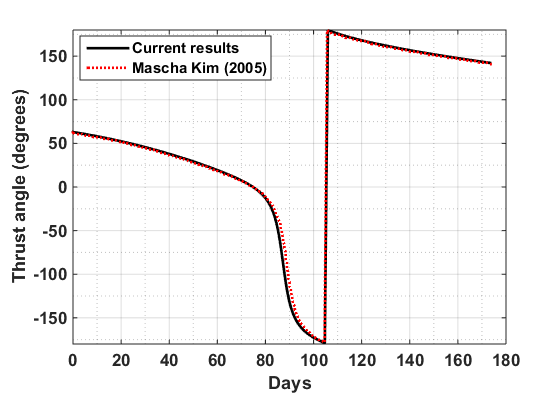
\includegraphics[width=0.65\linewidth]{Imgs/Results_Compare_bold.png}
	\vspace{-1.75mm}
	\caption{Comparison of obtained results with literature.}
\end{figure}	
\end{frame}

\begin{frame}
\frametitle{DE performance for Earth-Mars fuel optimal transfers}
\vspace{-2mm}
\begin{itemize}
	\item Different CR/F/NP combinations are values. (200 days, 2000s $I_{sp}$), $1mm/s^2$
\end{itemize}
\begin{figure}
	\vspace{-3.75mm}
	\centering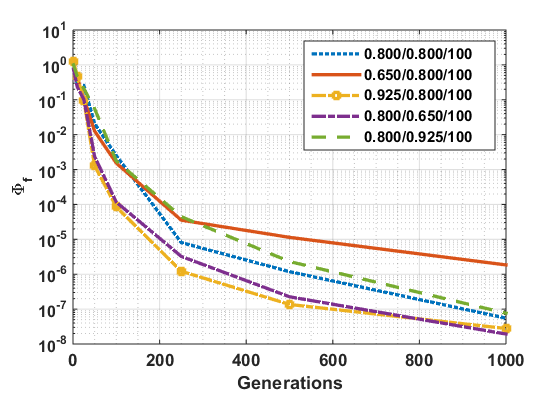
\includegraphics[width=0.60\linewidth]{Imgs/De_convgc_new.png}
%	\caption{}
\end{figure}
\vspace{-3.75mm}
It is observed that CR/F ratios greater than 1 are suitable for rapid convergence. CR=0.9 and F=0.8 has been chosen for further analysis.
\end{frame}

\begin{frame}
	\frametitle{Time optimal transfers}
	\vspace{-5mm}
	\begin{itemize}
		\item Earth-Mars transfer with varying initial acceleration levels.
	\end{itemize}
	\vspace{-6mm}
	\begin{figure}
		\centering\includegraphics[width=0.65\linewidth]{Imgs/Fuelfrac_isp.png}
	\end{figure}
Very low acceleration levels result in spiral transfers. These transfers take similar fuel fractions.
\end{frame}


\begin{frame}
	\frametitle{Earth-Mars fuel optimal transfers}
	\vspace{-3mm}
	\begin{itemize}
		\item NEP and SEP power models have been used.
		\item For small flight durations, NEP consumes much lower fuel than SEP.
		\item For large flight durations, all power models converge to the same fuel fraction.
	\end{itemize}
	\vspace{-3.25mm}
	\begin{figure}
		\centering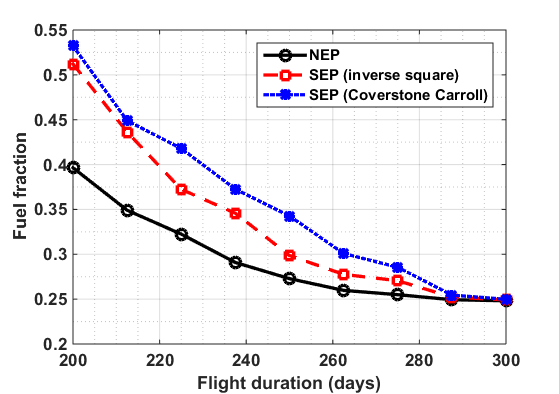
\includegraphics[width=0.60\linewidth]{Imgs/FuelOptParam.png}
	\end{figure}
\end{frame}

\begin{frame}
\frametitle{Earth-Mars fuel optimal transfers - Power models}
\vspace{-3.25mm}
\begin{figure}
	\centering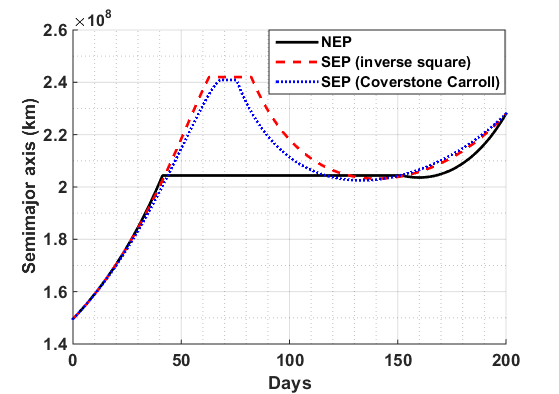
\includegraphics[width=0.60\linewidth]{Imgs/Semimaj_axis.png}
\end{figure}
\vspace{-3.00mm}
SEP models for a 200 day transfer show that solar power models tend to waste energy to satisfy the flight time constraint. This is due to reduced thrust at larger radii from the Sun.
\end{frame}

\begin{frame}
\frametitle{Sample trajectory - Earth to Mars - Heliocentric}
\vspace{-2.50mm}
\begin{itemize}
	\item 400 day fuel optimal transfer, 2000s $I_{sp}$, initial mass $1000kg$, thrust level $236mN$. (NEXT class thruster)
\end{itemize}
\begin{figure}
	\vspace{-1.50mm}
	\centering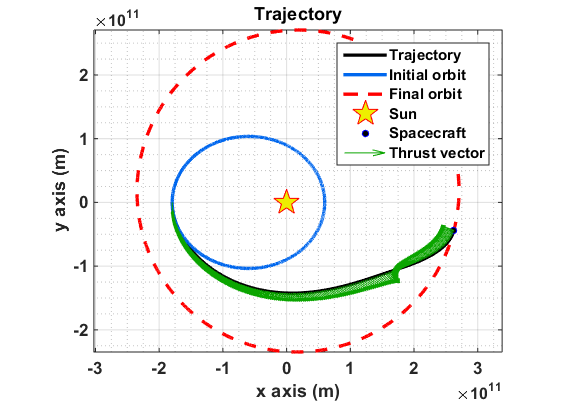
\includegraphics[width=0.70\linewidth]{Imgs/Sample_Traj.png}
\end{figure}
\end{frame}

%\begin{frame}
%	\frametitle{References}
%	\footnotesize{
%		\begin{thebibliography}{99} % Beamer does not support BibTeX so references must be inserted manually as below
%			\bibitem[Coverstone-Carroll, 1997]{covcarr} S. N. Williams and V. Coverstone-Carroll, Benefits of Solar Electric Propulsion for the Next Generation of
%			Planetary Exploration Missions.
%			\newblock \emph{The Journal of the Astronautical Sciences, 45(2):143-160, April-June 1997} 
%			
%			\bibitem[Kirk (2012)]{kirk} Donald E. Kirk, Optimal Control Theory: An Introduction.
%			\newblock \emph{Courier Corporation (2012)}
%			
%			\bibitem[Storn and Price, 1997]{stoprice} Storn. Rainer and Price. Kenneth, Differential Evolution − A Simple and Efficient Heuristic for Global Optimization over Continuous Spaces.
%			\newblock \emph{Journal of Global Optimization 11, no. 4 (1997): 341-359.}
%		\end{thebibliography}
%	}
%\end{frame}

%\begin{frame}
%\frametitle{Bullet Points}
%\begin{itemize}
%\item Lorem ipsum dolor sit amet, consectetur adipiscing elit
%\item Aliquam blandit faucibus nisi, sit amet dapibus enim tempus eu
%\item Nulla commodo, erat quis gravida posuere, elit lacus lobortis est, quis porttitor odio mauris at libero
%\item Nam cursus est eget velit posuere pellentesque
%\item Vestibulum faucibus velit a augue condimentum quis convallis nulla gravida
%\end{itemize}
%\end{frame}

%------------------------------------------------

%\begin{frame}
%\frametitle{Blocks of Highlighted Text}
%\begin{block}{Block 1}
%Lorem ipsum dolor sit amet, consectetur adipiscing elit. Integer lectus nisl, ultricies in feugiat rutrum, porttitor sit amet augue. Aliquam ut tortor mauris. Sed volutpat ante purus, quis accumsan dolor.
%\end{block}

%\begin{block}{Block 2}
%Pellentesque sed tellus purus. Class aptent taciti sociosqu ad litora torquent per conubia nostra, per inceptos himenaeos. Vestibulum quis magna at risus dictum tempor eu vitae velit.
%\end{block}
%
%\begin{block}{Block 3}
%Suspendisse tincidunt sagittis gravida. Curabitur condimentum, enim sed venenatis rutrum, ipsum neque consectetur orci, sed blandit justo nisi ac lacus.
%\end{block}
%\end{frame}

%------------------------------------------------

%\begin{frame}
%\frametitle{Multiple Columns}
%\begin{columns}[c] % The "c" option specifies centered vertical alignment while the "t" option is used for top vertical alignment
%
%\column{.45\textwidth} % Left column and width
%\textbf{Heading}
%\begin{enumerate}
%\item Statement
%\item Explanation
%\item Example
%\end{enumerate}
%
%\column{.5\textwidth} % Right column and width
%Lorem ipsum dolor sit amet, consectetur adipiscing elit. Integer lectus nisl, ultricies in feugiat rutrum, porttitor sit amet augue. Aliquam ut tortor mauris. Sed volutpat ante purus, quis accumsan dolor.
%
%\end{columns}
%\end{frame}

%------------------------------------------------
%\section{Second Section}
%%------------------------------------------------
%
%\begin{frame}
%\frametitle{Table}
%\begin{table}
%\begin{tabular}{l l l}
%\toprule
%\textbf{Treatments} & \textbf{Response 1} & \textbf{Response 2}\\
%\midrule
%Treatment 1 & 0.0003262 & 0.562 \\
%Treatment 2 & 0.0015681 & 0.910 \\
%Treatment 3 & 0.0009271 & 0.296 \\
%\bottomrule
%\end{tabular}
%\caption{Table caption}
%\end{table}
%\end{frame}
%
%%------------------------------------------------
%
%\begin{frame}
%\frametitle{Theorem}
%\begin{theorem}[Mass--energy equivalence]
%$E = mc^2$
%\end{theorem}
%\end{frame}
%
%%------------------------------------------------
%
%\begin{frame}[fragile] % Need to use the fragile option when verbatim is used in the slide
%\frametitle{Verbatim}
%\begin{example}[Theorem Slide Code]
%\begin{verbatim}
%\begin{frame}
%\frametitle{Theorem}
%\begin{theorem}[Mass--energy equivalence]
%$E = mc^2$
%\end{theorem}
%\end{frame}\end{verbatim}
%\end{example}
%\end{frame}
%
%%------------------------------------------------
%
%\begin{frame}
%\frametitle{Figure}
%Uncomment the code on this slide to include your own image from the same directory as the template .TeX file.
%%\begin{figure}
%%\includegraphics[width=0.8\linewidth]{test}
%%\end{figure}
%\end{frame}
%
%%------------------------------------------------
%
%\begin{frame}[fragile] % Need to use the fragile option when verbatim is used in the slide
%\frametitle{Citation}
%An example of the \verb|\cite| command to cite within the presentation:\\~
%
%This statement requires citation \cite{p1}.
%\end{frame}

%------------------------------------------------

%\begin{frame}
%\frametitle{References}
%\footnotesize{
%\begin{thebibliography}{99} % Beamer does not support BibTeX so references must be inserted manually as below
%\bibitem[Smith, 2012]{p1} John Smith (2012)
%\newblock Title of the publication
%\newblock \emph{Journal Name} 12(3), 45 -- 678.
%\end{thebibliography}
%}
%\end{frame}

%------------------------------------------------

\begin{frame}
\Huge{\centerline{Thank You}}
\end{frame}

%----------------------------------------------------------------------------------------

\end{document} 